\subsection{Number of Athletes by Age}\label{subsec:number-of-athletes-by-age}

To determine to determine the average age of the athletes, we can run the following SQL query:

\begin{minted}{sql}
SELECT AVG(age(birthdate))
FROM annp_final.athlete;
\end{minted}

From this, we can see that the average age of the athletes is 46 years, 6 months and 31 days.

We can also determine who's the youngest athlete by running the following SQL query:

\begin{minted}{sql}
SELECT *
FROM annp_final.athlete
ORDER BY age(birthdate) ASC
LIMIT 1;
\end{minted}

\begin{itemize}
    \item \textbf{Name:} Ana Mónica Eloi
    \item \textbf{Gender:} Female
    \item \textbf{Birthdate:} 29/12/1996
    \item \textbf{Age:} 25 years
\end{itemize}

On the other hand, we can learn information about the oldest athlete by running the following SQL query:

\begin{minted}{sql}
SELECT *
FROM annp_final.athlete
ORDER BY age(birthdate) DESC
LIMIT 1;
\end{minted}

\begin{itemize}
    \item \textbf{Name:} Virgílio Zacarias Costa
    \item \textbf{Gender:} Male
    \item \textbf{Birthdate:} 21/07/1931
    \item \textbf{Age:} 90 years
\end{itemize}

Finally, to determine the number of athletes by age, we can run the following SQL query using the PostgreSQL's built-in
\texttt{age} function:

\begin{minted}{sql}
SELECT COUNT(*), EXTRACT(YEAR FROM age(birthdate)) AS age
FROM annp_final.athlete
GROUP BY age
ORDER BY age ASC;
\end{minted}

We can then plot the result, as illustrated in \cref{fig:athletesbynation}.

\begin{figure}[H]
    \centering
    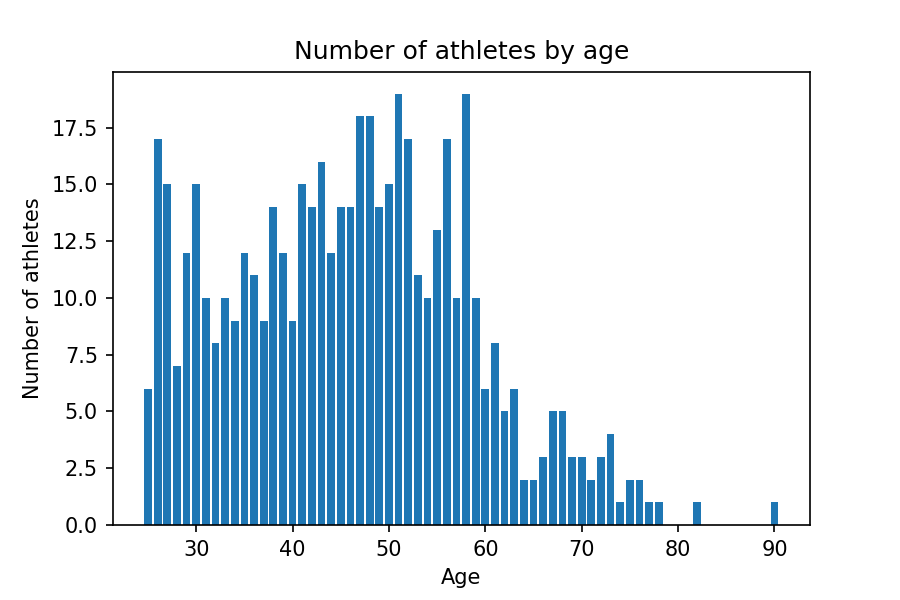
\includegraphics[width=\textwidth]{img/athletesbyage}
    \caption{Number of athletes by age}
    \label{fig:athletesbyage}
\end{figure}

\subsection{Number of Athletes by Nation}\label{subsec:number-of-athletes-by-nation}

To determine the number of athletes by nation, we can run the following SQL query:

\begin{minted}{sql}
SELECT COUNT(*) nationCount, nation
FROM annp_final.athlete
GROUP BY nation
ORDER BY nationCount ASC;
\end{minted}

We can then plot the result, as illustrated in \cref{fig:athletesbynation}.

\begin{figure}[H]
    \centering
    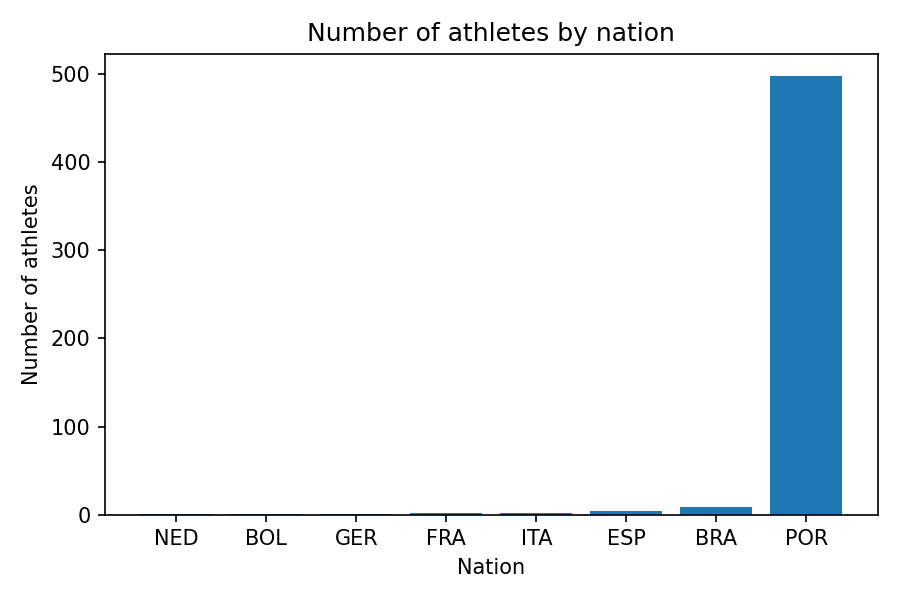
\includegraphics[width=.8\textwidth]{img/athletesbynation}
    \caption{Number of athletes by nation}
    \label{fig:athletesbynation}
\end{figure}

To have another perspective, we can also plot in a pie chart, as illustrated in \cref{fig:athletesbynation-pie}.

\begin{figure}[H]
    \centering
    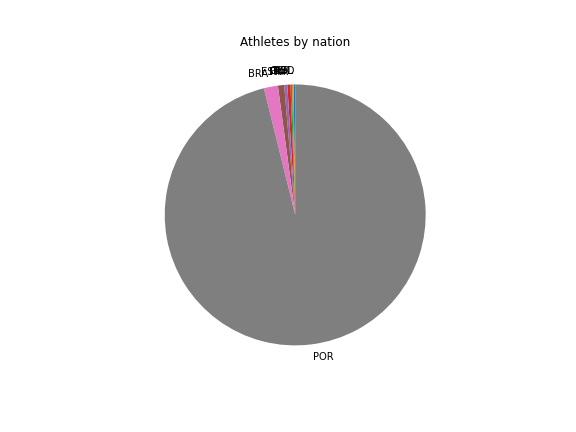
\includegraphics[width=.8\textwidth]{img/athletesbynation-piechart}
    \caption{Number of athletes by nation}
    \label{fig:athletesbynation-pie}
\end{figure}

\subsection{Number of Athletes by Gender}\label{subsec:number-of-athletes-by-gender}

To determine the number of athletes by gender, we can run the following SQL query:

\begin{minted}{sql}
SELECT COUNT(*), gender
FROM annp_final.athlete
GROUP BY gender;
\end{minted}

We can then plot the result, as illustrated in \cref{fig:athletesbygender}.

\begin{figure}[H]
    \centering
    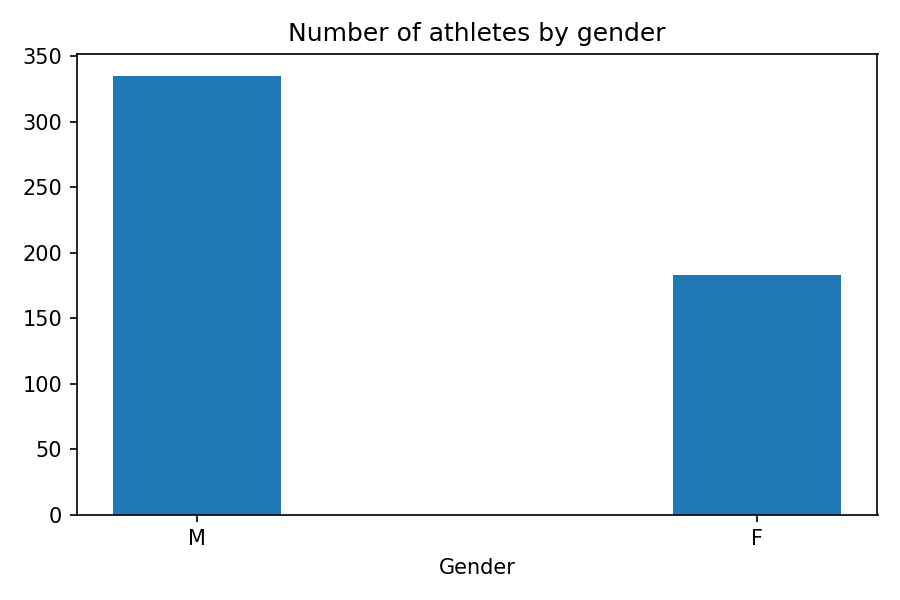
\includegraphics[width=.35\textwidth]{img/athletesbygender}
    \caption{Number of athletes by gender}
    \label{fig:athletesbygender}
\end{figure}

We can also plot this in a pie chart, as illustrated in \cref{fig:athletesbygender-pie}.

\begin{figure}[H]
    \centering
    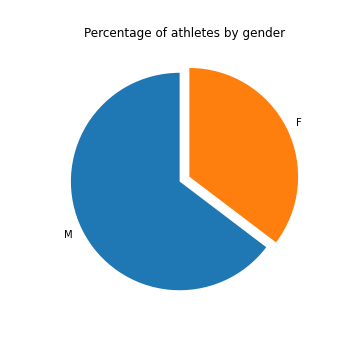
\includegraphics[width=.45\textwidth]{img/athletesbygender-pie}
    \caption{Percentage of athletes by gender}
    \label{fig:athletesbygender-pie}
\end{figure}

\subsection{Number of Events by Gender}\label{subsec:number-of-events-by-gender}

To determine the number of events by gender, we can run the following SQL query:

\begin{minted}{sql}
SELECT COUNT(*), gender
FROM annp_final.event
GROUP BY gender;
\end{minted}

We can then plot the result, as illustrated in \cref{fig:eventsbygender}.

\begin{figure}[H]
    \centering
    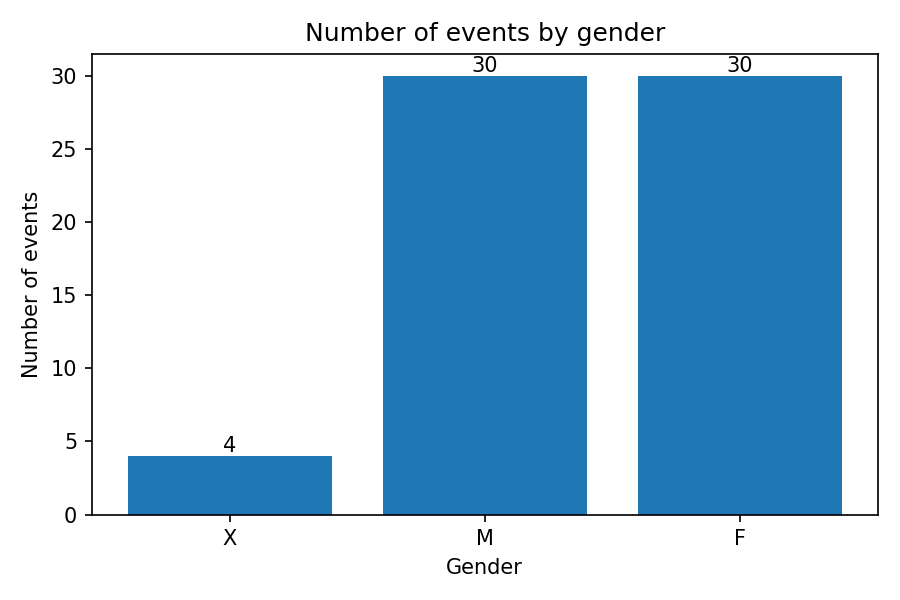
\includegraphics[width=.35\textwidth]{img/eventsbygender}
    \caption{Number of events by gender}
    \label{fig:eventsbygender}
\end{figure}

Here, the value \texttt{X} refers to events that allow athletes from both genders to participate.
We can also plot this in a pie chart, as illustrated in \cref{fig:eventsbygender-pie}.

\begin{figure}[H]
    \centering
    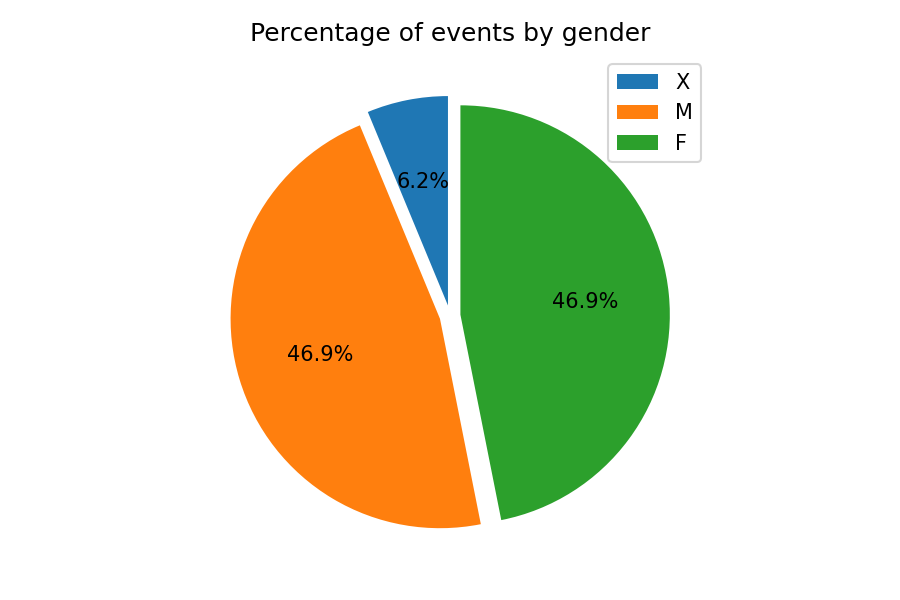
\includegraphics[width=.45\textwidth]{img/eventsbygender-pie}
    \caption{Percentage of events by gender}
    \label{fig:eventsbygender-pie}
\end{figure}

\subsection{Number of Clubs by Nation}\label{subsec:number-of-clubs-by-nation}

We can determine the number of clubs by each nation by running the following SQL query:

\begin{minted}{sql}
SELECT nation, COUNT(*) AS nationCount
FROM annp_final.club
GROUP BY nation
ORDER BY nationCount ASC;
\end{minted}

Plotting the result in a bar chart, we have the following:

\begin{figure}[H]
    \centering
    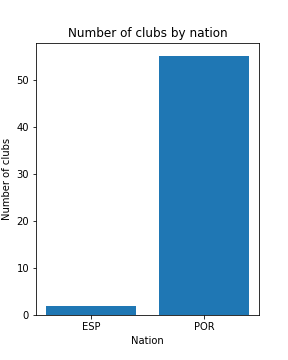
\includegraphics[width=.35\textwidth]{img/clubsbynation}
    \caption{Number of clubs by nation}
    \label{fig:clubs-by-nation}
\end{figure}

\subsection{Number of Clubs by Region}\label{subsec:number-of-clubs-by-region}

To determine the number of clubs per each region in Portugal, we can run the following SQL query:

\begin{minted}{sql}
SELECT region, COUNT(*) AS regionCount
FROM annp_final.club
WHERE region SIMILAR TO '[A-Z]+'
GROUP BY region
ORDER BY regionCount ASC;
\end{minted}

Plotting the result of the query in a bar chart we have the following:

\begin{figure}[H]
    \centering
    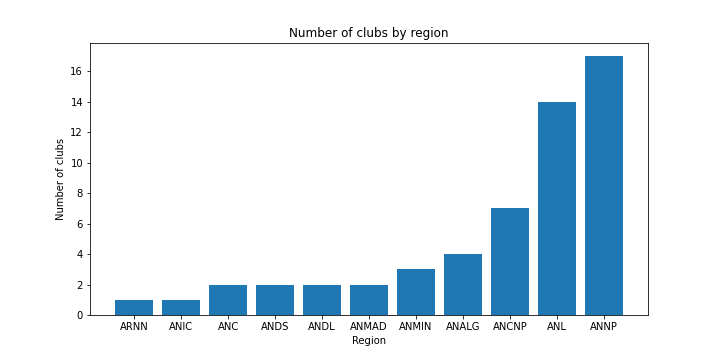
\includegraphics[width=.85\textwidth]{img/clubsbyregion}
    \caption{Number of clubs by region}
    \label{fig:clubs-by-region}
\end{figure}

Here, it is worth noting that this query only considers the portuguese clubs, because each is identified by uppercase
letters only.
Spanish regions, on the other hand, are identified with numbers, which means that if we want to run the previous query
considering only spanish regions, we only have to replace \texttt{WHERE region SIMILAR TO '[A-Z]+'} with
\texttt{WHERE region SIMILAR TO '[0-9]+'}, as shown bellow:

\begin{minted}{sql}
SELECT region, COUNT(*) AS regionCount
FROM annp_final.club
WHERE region SIMILAR TO '[0-9]+'
GROUP BY region
ORDER BY regionCount ASC;
\end{minted}

However, this has a downside in the sense that we have no way of knowing which regions these values \texttt{10114} and
\texttt{11115} refer to.
Ploting the result in a bar plot, we have the following:

\begin{figure}[H]
    \centering
    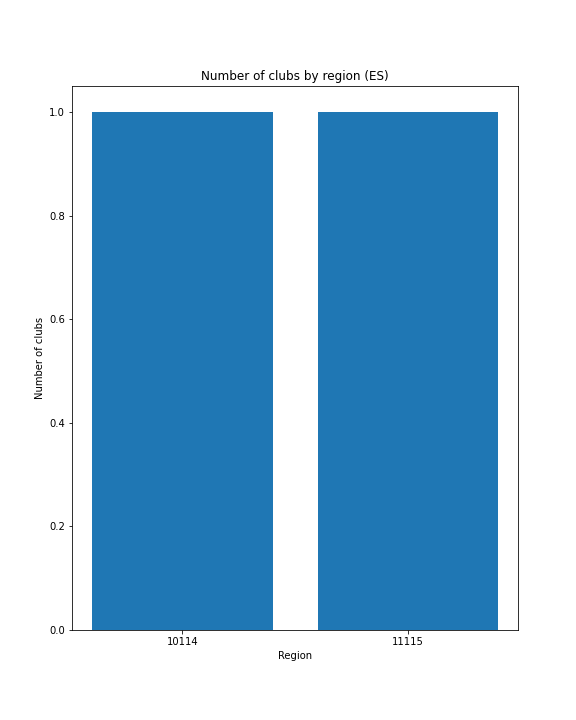
\includegraphics[width=.5\textwidth]{img/clubsbyregion-es}
    \caption{Number of clubs by region (ES)}
    \label{fig:clubs-by-region-es}
\end{figure}

We can also plot this a pie chart, which gives us the following:

\begin{figure}[H]
    \centering
    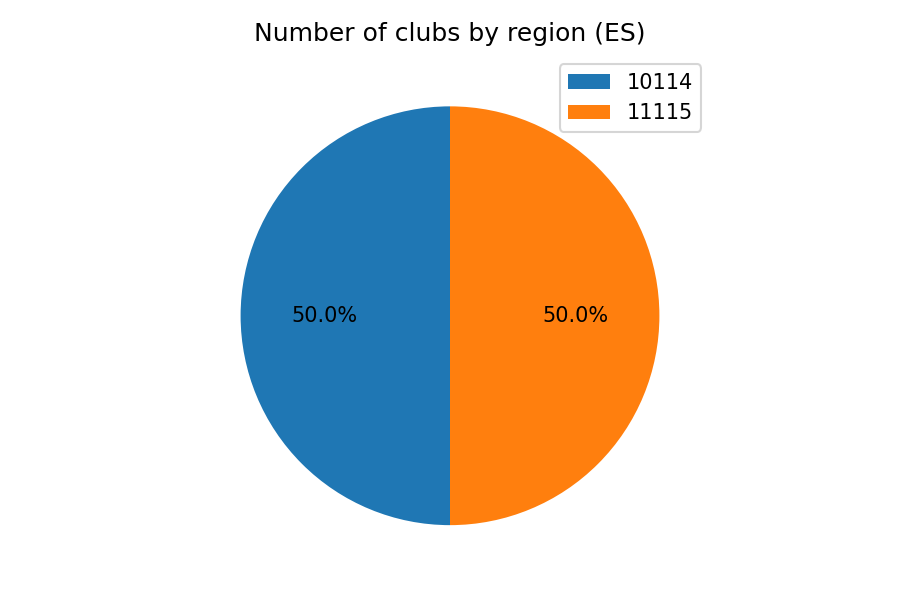
\includegraphics[width=.5\textwidth]{img/clubsbyregion-es-pie}
    \caption{Number of clubs by region (ES)}
    \label{fig:clubs-by-region-es-pie}
\end{figure}

\subsection{Events by time}

To find out the most frequent time for swimming events (\textit{i.e.} the time at which most of the events take place),
we can run the following SQL query:

\begin{minted}{sql}
SELECT time, COUNT(*) AS eventCount
FROM annp_final.event
GROUP BY time
ORDER BY time DESC;
\end{minted}

Plotting the result in a bar plot, we have the following:

\begin{figure}[H]
    \centering
    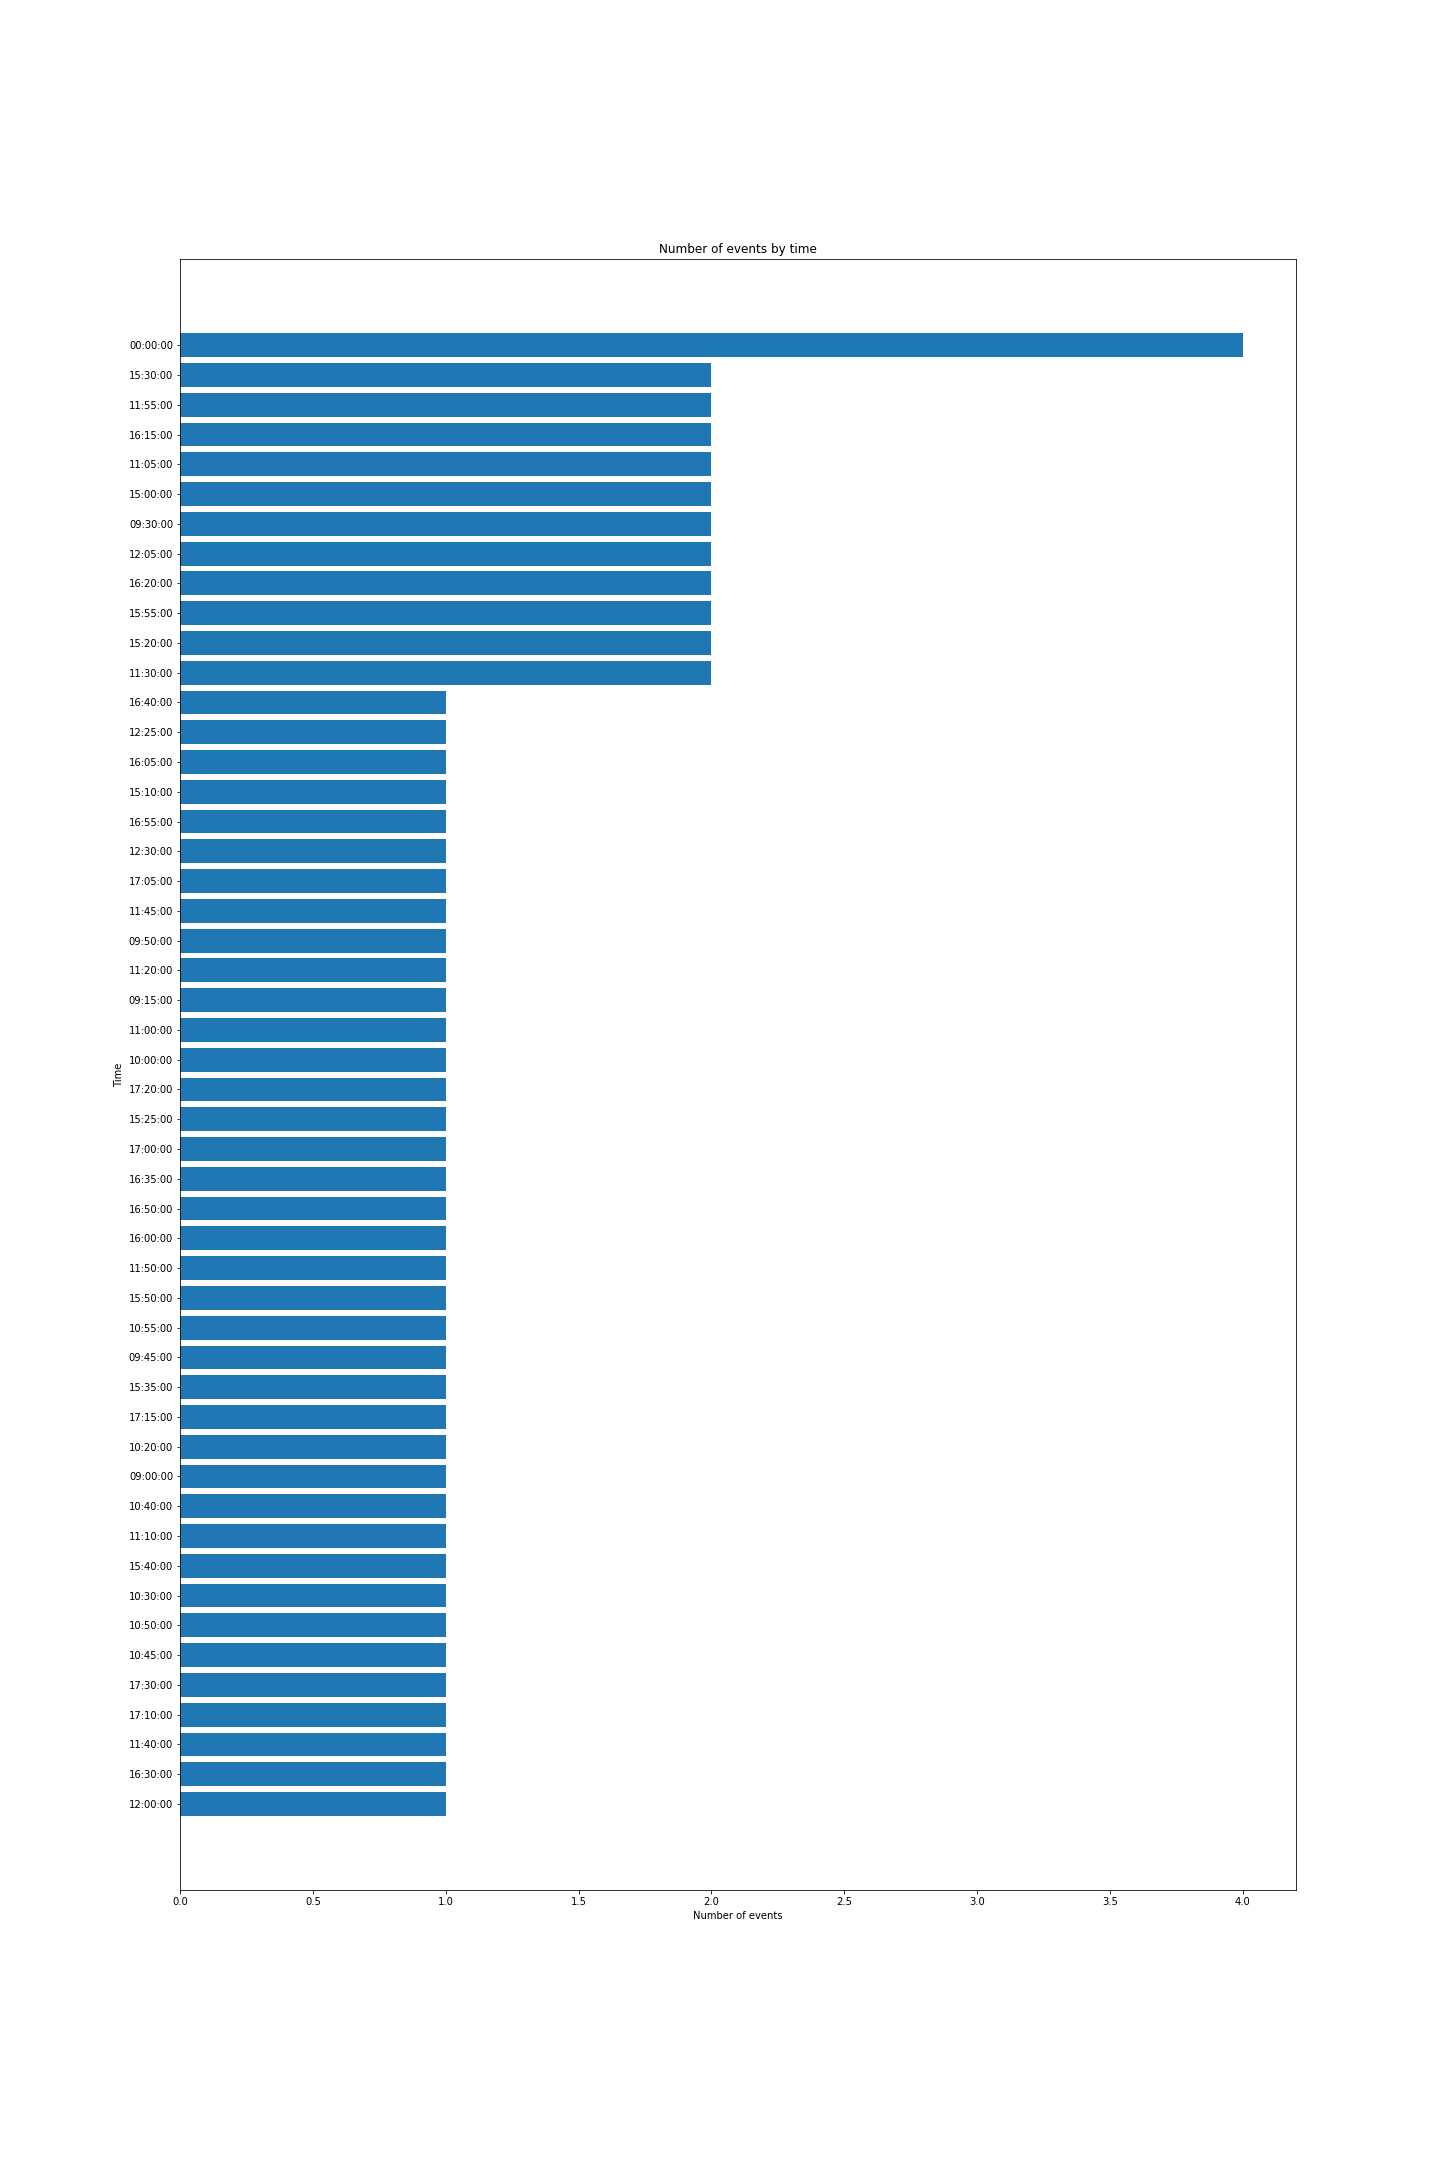
\includegraphics[width=\textwidth]{img/eventsbytime}
    \caption{Number of events by time}
    \label{fig:events-by-time}
\end{figure}

\subsection{Swimming Styles}

\textcolor{red}{COMPLETAR COM TEXTO (style com mais distance) É FRESSTYLE}.

\begin{minted}{sql}
SELECT *
FROM annp_final.swimstyle
ORDER BY distance DESC
LIMIT 1;
\end{minted}

\textcolor{red}{COMPLETAR COM TEXTO (style com menos distance) FLY}.

\begin{minted}{sql}
SELECT *
FROM annp_final.swimstyle
ORDER BY distance ASC
LIMIT 1;
\end{minted}

\subsection{Results}

\subsubsection{Average Swim Time}

\textcolor{red}{COMPLETAR COM TEXTO (resultado = 00:02:23.769068)}.

\begin{minted}{sql}
SELECT AVG(swimtime)
FROM annp_final.result;
\end{minted}

\subsubsection{Average Number of Points}

\textcolor{red}{COMPLETAR COM TEXTO (resultado = 340)}.
\begin{minted}{sql}
SELECT AVG(points)::numeric(10, 1)
FROM annp_final.result;
\end{minted}

\subsection{Club facts statistics}

\begin{minted}{sql}
SELECT 
CASE GROUPING(cd.meetid)
    WHEN 1 THEN 'all_meets'
    ELSE cd.meetid
END AS "Tournament",
CASE GROUPING(c.code)
    WHEN 1 THEN 'all_clubs'
    ELSE c.code
END AS "Team",
   ROUND(AVG(average_age), 0) AS "Average Age",
   ROUND(AVG(average_swimtime), 2) AS "Average Swimtime",
   ROUND(SUM(total_points)) AS "Total Points",
   ROUND(SUM(number_of_players)) AS "Total Players"
FROM (
    SELECT CAST(meetid AS VARCHAR(255)),
       clubid,
       average_age,
       total_points,
       average_swimtime,
       number_of_players
    FROM annp_final.club_defacto) cd
JOIN annp_final.club c ON c.clubid = cd.clubid
GROUP BY CUBE (cd.meetid, c.code);
\end{minted}


\begin{figure}[H]
    \centering
    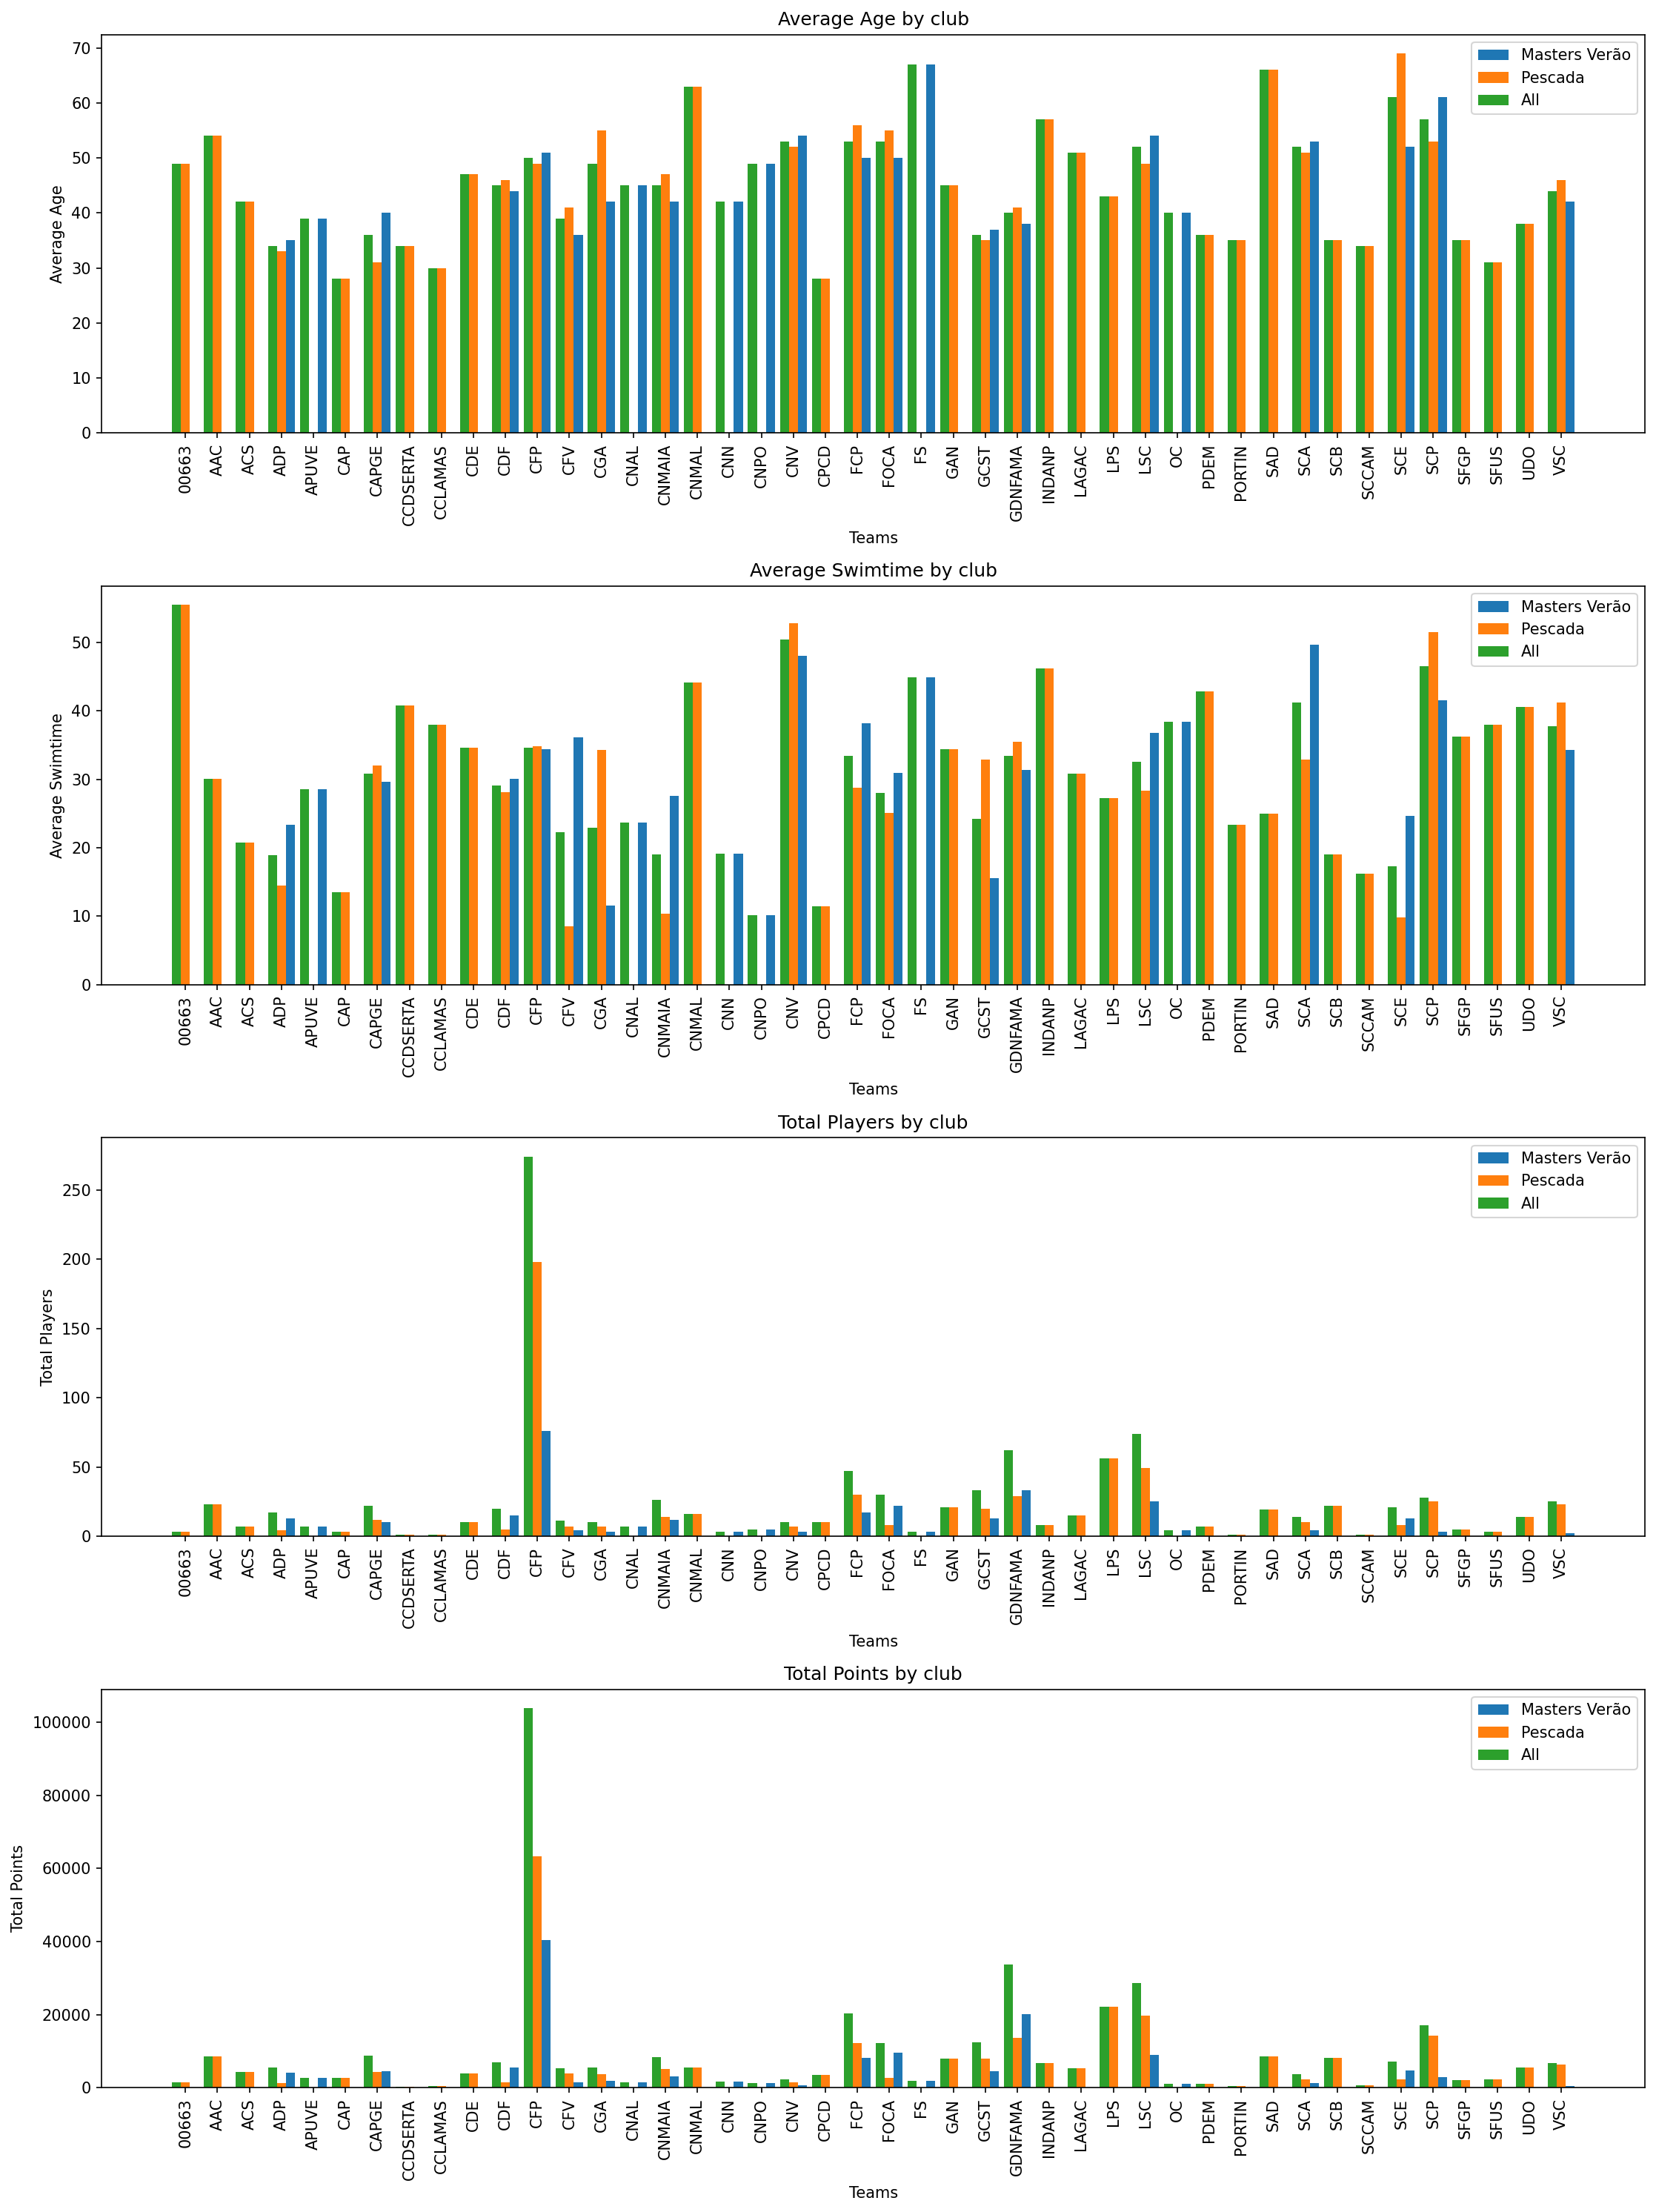
\includegraphics[width=\textwidth]{img/clubdefactostats.png}
    \caption{Statistics from fact Club table.}
    \label{fig:clubs_fact}
\end{figure}

\subsection{Athlete facts statistics}

\begin{minted}{sql}
SELECT
    CASE GROUPING(a.firstname)
        WHEN 1 THEN 'all_players'
        ELSE a.firstname
    END AS "Athletes",
    CASE GROUPING(af.meetid)
        WHEN 1 THEN 'all_meets'
        ELSE af.meetid
    END AS "Tournament",
    ROUND(AVG(average_points), 2) AS "Average Points",
    ROUND(AVG(average_distance), 2) AS "Average Distance",
    ROUND(AVG(average_swimtime), 2) AS "Average Swimtime"
FROM (
    SELECT
        athleteid,
        CAST(meetid as VARCHAR(255)),
        average_points,
        average_distance,
        average_swimtime
    FROM annp_final.athlete_defacto) af
JOIN annp_final.athlete a ON a.athleteid = af.athleteid
GROUP BY CUBE (a.firstname, af.meetid)
ORDER BY "Average Points" DESC
LIMIT 50;
\end{minted}


\begin{figure}[H]
    \centering
    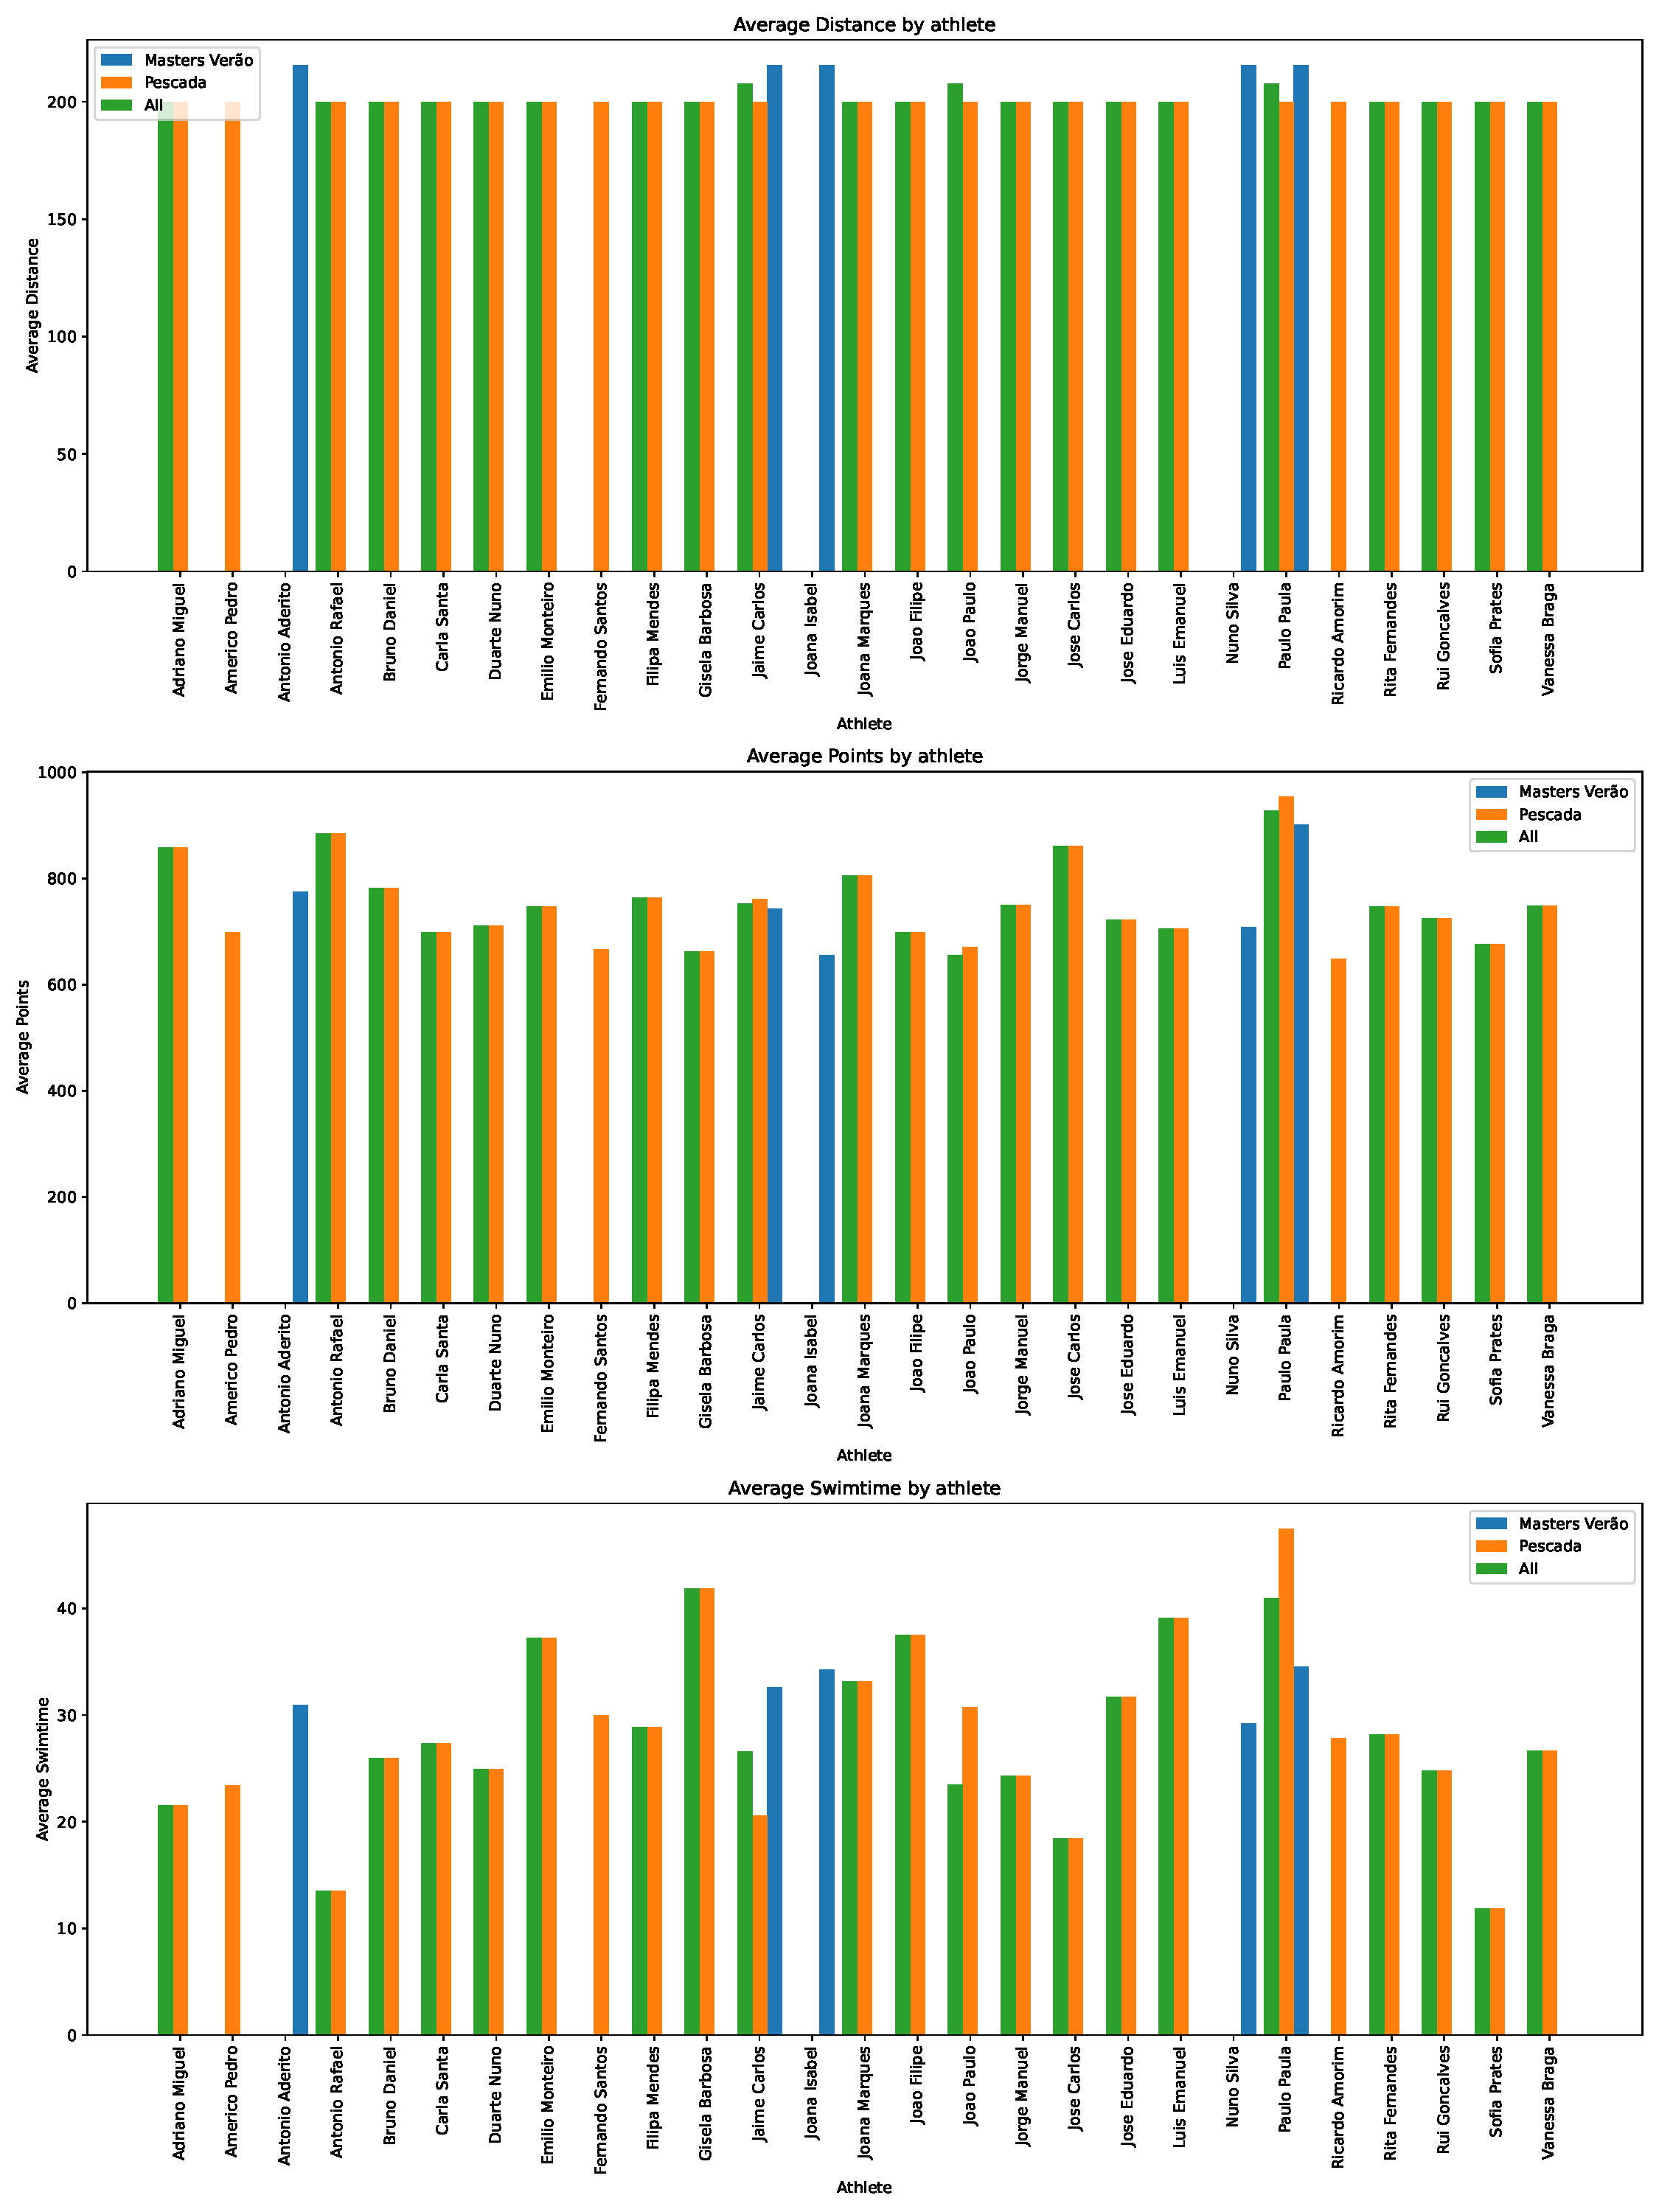
\includegraphics[width=\textwidth]{img/athletefact.pdf}
    \caption{Statistics from fact Club table.}
    \label{fig:athlete_fact}
\end{figure}